%% 
%% Created in 2018 by Martin Slapak
%%
%% Based on file for NRP report LaTeX class by Vit Zyka (2008)
%%

\documentclass[english]{mvi-report}

\usepackage[utf8]{inputenc} 
\usepackage[style=iso-numeric]{biblatex}

\addbibresource{bibliography.bib}


\title{Utilizing Earthformer Transformer for Radar Data Extraction from Satellite Imagery}

\author{Filip Miškařík}
\affiliation{FIT ČVUT}
\email{miskafil@fit.cvut.cz}

\def\file#1{{\tt#1}}

\begin{document}

\maketitle

%%%%%%%%%%%%%%%%%%%%%%%%%%%%%%%%%%%%%%%%%%%%%%%%%%%%%%%%%%%%%%%%%%%%%%%%%%%%%%%%
\section{Introduction}
Precipitation nowcasting is a crucial task in meteorology that aims to give a precise short-term prediction of rainfall intensity in a local region. These predictions are usually based on data from weather radars, which directly capture the position and intensity of rainfall with reflections of electromagnetic waves \cite{radar_article}. However, in many parts of the world, radar data is not available, because weather radars are very sophisticated and expensive to build and maintain \cite{guildelines_for_nowcasting}.

Weather satellites, on the other hand, can provide observations for locations without ground radars. Satellites capture images with high spatiotemporal resolution in both visible and infrared spectrum. However, unlike weather radars, satellites don't directly measure rainfall and are therefore not suitable for precipitation nowcasting.

We attempt to bridge the gap between these two problems. By utilizing data from the SEVIR dataset, we translate satellite to radar data (sat2rad translation), which can then serve as further input for nowcasting models.

Image translation tasks usually utilize the convolutional neural network (CNN) architecture, an example being the ubiquitous U-Net model \cite{unet}. Models for nowcasting extend the CNN with recurrent neural networks (RNN) to allow for processing sequences of images. In \cite{earthformer}, Gao et al. presented Earthformer, a model for nowcasting that does not utilize the CNN architecture and is instead based on the Transformer model.

The goal of this work is to utilize Earthformer for extracting synthetic radar data from satellite imagery. We then compare the performance of Earthformer to the U-Net. For simplicity, we only focus on translating individual images from satellite to radar without doing any sequence forecasting.

%%%%%%%%%%%%%%%%%%%%%%%%%%%%%%%%%%%%%%%%%%%%%%%%%%%%%%%%%%%%%%%%%%%%%%%%%%%%%%%%
\section{Dataset}
The SEVIR dataset is a collection of around 12 000 spatially and temporally aligned weather events. These events are comprised of 4-hour sequences sampled every 5-minutes across a 384x384 km area somewhere in the USA during the years 2018 and 2019. The images in SEVIR contain 5 different image channels: 0.6 $\mu m$ visible satellite channel (\texttt{vis}), 6.9 $\mu m$ and 10.7 $\mu m$ satellite infrared channels (\texttt{ir069}, \texttt{ir107}), a radar mosaic of vertically integrated liquid (\texttt{vil}), and total lightning flashes collected by the GOES-16 geostationary lightning mapper (GLM) (\texttt{lght}) \cite{SEVIR}. The lightning modality is the only non-image type, and is represented by a continuous collection of GLM lightning flashes captured in the 4 hour time window.

To create our dataset for sat2rad prediction, we extracted all sequences into individual images. We used either $\{\texttt{ir069}, \texttt{ir107}\}$ or $\{\texttt{ir069}, \texttt{ir107}, \texttt{lght}\}$ as the input channels and \texttt{vil} images as the ground truth. The visible spectrum satellite images were not utilized in order to achieve same performance during the day and night and also to reduce storage requirements as these images take up most of the 1 TB dataset. We then followed the same preprocessing steps as used by authors of the SEVIR dataset in \cite{SEVIR}.

The \texttt{lght} data was converted to an image by binning 5 minutes of flashes prior to \texttt{ir069} and \texttt{ir107} onto a 48 x 48 pixel grid. The \texttt{lght} and \texttt{vil} input images were then upscaled and downscaled respectively to the common size of 192x192 of the satellite data. Each channel was then normalized by subtracting their mean and dividing by their standard deviation computed over the training set. These images were then passed to our neural networks.

We obtained approximately 570 000 individual images, which were then split into train, validation and test sets with the ratio of 70:20:10.

%%%%%%%%%%%%%%%%%%%%%%%%%%%%%%%%%%%%%%%%%%%%%%%%%%%%%%%%%%%%%%%%%%%%%%%%%%%%%%%%
\section{Model architecture \& training setup}
The Earthformer is a model designed for spatiotemporal prediction based on the Transformer model with a hierarchical encoder-decoder architecture, where the input observations are encoded as a hierarchy of hidden states and then decoded to the prediction target \cite{earthformer}.

To combat the high computational and memory requirements of the self-attention mechanism on high-dimensional weather data, the model decomposes the input into smaller cuboids, applies self-attention within each cuboid in parallel and then merges the cuboids back. To allow for communication between the cuboids, the model utilizes global vectors, which convey the global dynamics of the system.
Multiple Cuboid Attention layers are then stacked and combined with cross-attention to the global vectors to form the resulting model. \cite{earthformer}

In our experiments, we used the Earthformer with 4 attention heads and 8 global vectors. 

For comparison, we trained a 3D U-Net with 5 encoder blocks with 32, 64, 128, 256 and 512 3x3 filters, followed by 4 decoder blocks and a final 2D convolutional layer with 1x1 filter that outputs a single channel image.

Both networks were trained with the Adam optimizer with a learning rate of 0.001. The loss function minimized during training was MSE, but we also tried training both models with MAE. The training process was set to a maximum of 50 epochs with early stopping used to avoid overfitting.

%%%%%%%%%%%%%%%%%%%%%%%%%%%%%%%%%%%%%%%%%%%%%%%%%%%%%%%%%%%%%%%%%%%%%%%%%%%%%%%%
\section{Results}

\begin{table}
    \centering
    \begin{tabular}{l||ccc}
        Model & MAE & MSE & CSI ($\uparrow$) \\
        \hline\hline
        Earthformer 2 chan. & 11.77 & 525.2 & 0.336 \\
        Earthformer 3 chan. & \textbf{11.14} & 472.4 & 0.378 \\
        U-Net 2 channels & 11.39 & 506.4 & 0.341 \\
        U-Net 3 channels & 11.27 & \textbf{455.8} & \textbf{0.387} \\
    \end{tabular}
    \caption{Performance of our models on the test set.}
    \label{tab:performance_2vs3_channels}
\end{table}

We evaluated our models on three metrics -- MSE and MAE, which calculate a per-pixel error and Critical Success Index (CSI), which binarizes the output and target with some threshold value and then computes the metric as $\textrm{CSI} = \frac{\textrm{TP}}{\textrm{TP} + \textrm{TN} + \textrm{FP}}$ \cite{forecast_glossary}. We took the ame approach as in \cite{SEVIR} and calculated CSI with thresholds [16, 74, 133, 160, 181, 219] and then computed an average across all thresholds to get the final score.


Table \ref{tab:performance_2vs3_channels} shows the performance of both Earthformer and U-Net models trained with MSE loss function and either 2- or 3-channel inputs. The addition of the third channel with lightning data improved performance for both Earthformer and U-Net. Overall, U-Net with 3 channel inputs achieved the best MSE and average CSI, but the 3-channel Earthformer was best in MAE. 

Visually, predictions from the Earthformer in Figure \ref{fig:predictions} appear more smoothed than those from the U-Net. The visualizations also show that the lightning data helps the models identify areas with most intense precipitation.

We also subsequently trained the 3-channel models with MAE as the loss function. As shown in \ref{tab:prformance_MSEvsMAE}, this resulted in improvement in all three metrics for the Earthformer and improvement in MAE and CSI for the U-Net. Further experimentation could also try training both models with $\mathcal{L}_{1,2}$ loss.

\begin{table}
    \centering
    \begin{tabular}{l||ccc}
        Model & MAE & MSE & CSI ($\uparrow$) \\
        \hline\hline
        Earthformer MAE & 10.82 & 471.8 & 0.385 \\
        Earthformer MSE & 11.14 & 472.4 & 0.378 \\
        \hline
        U-Net MAE & \textbf{10.54} & 509.3 & \textbf{0.398} \\
        U-Net MSE & 11.27 & \textbf{455.8} & 0.387 \\
    \end{tabular}
    \caption{Performance of the 3-channel models when trained with MSE and MAE loss functions.}
    \label{tab:prformance_MSEvsMAE}
\end{table}

\begin{figure*}[ht]
  \centering\leavevmode
  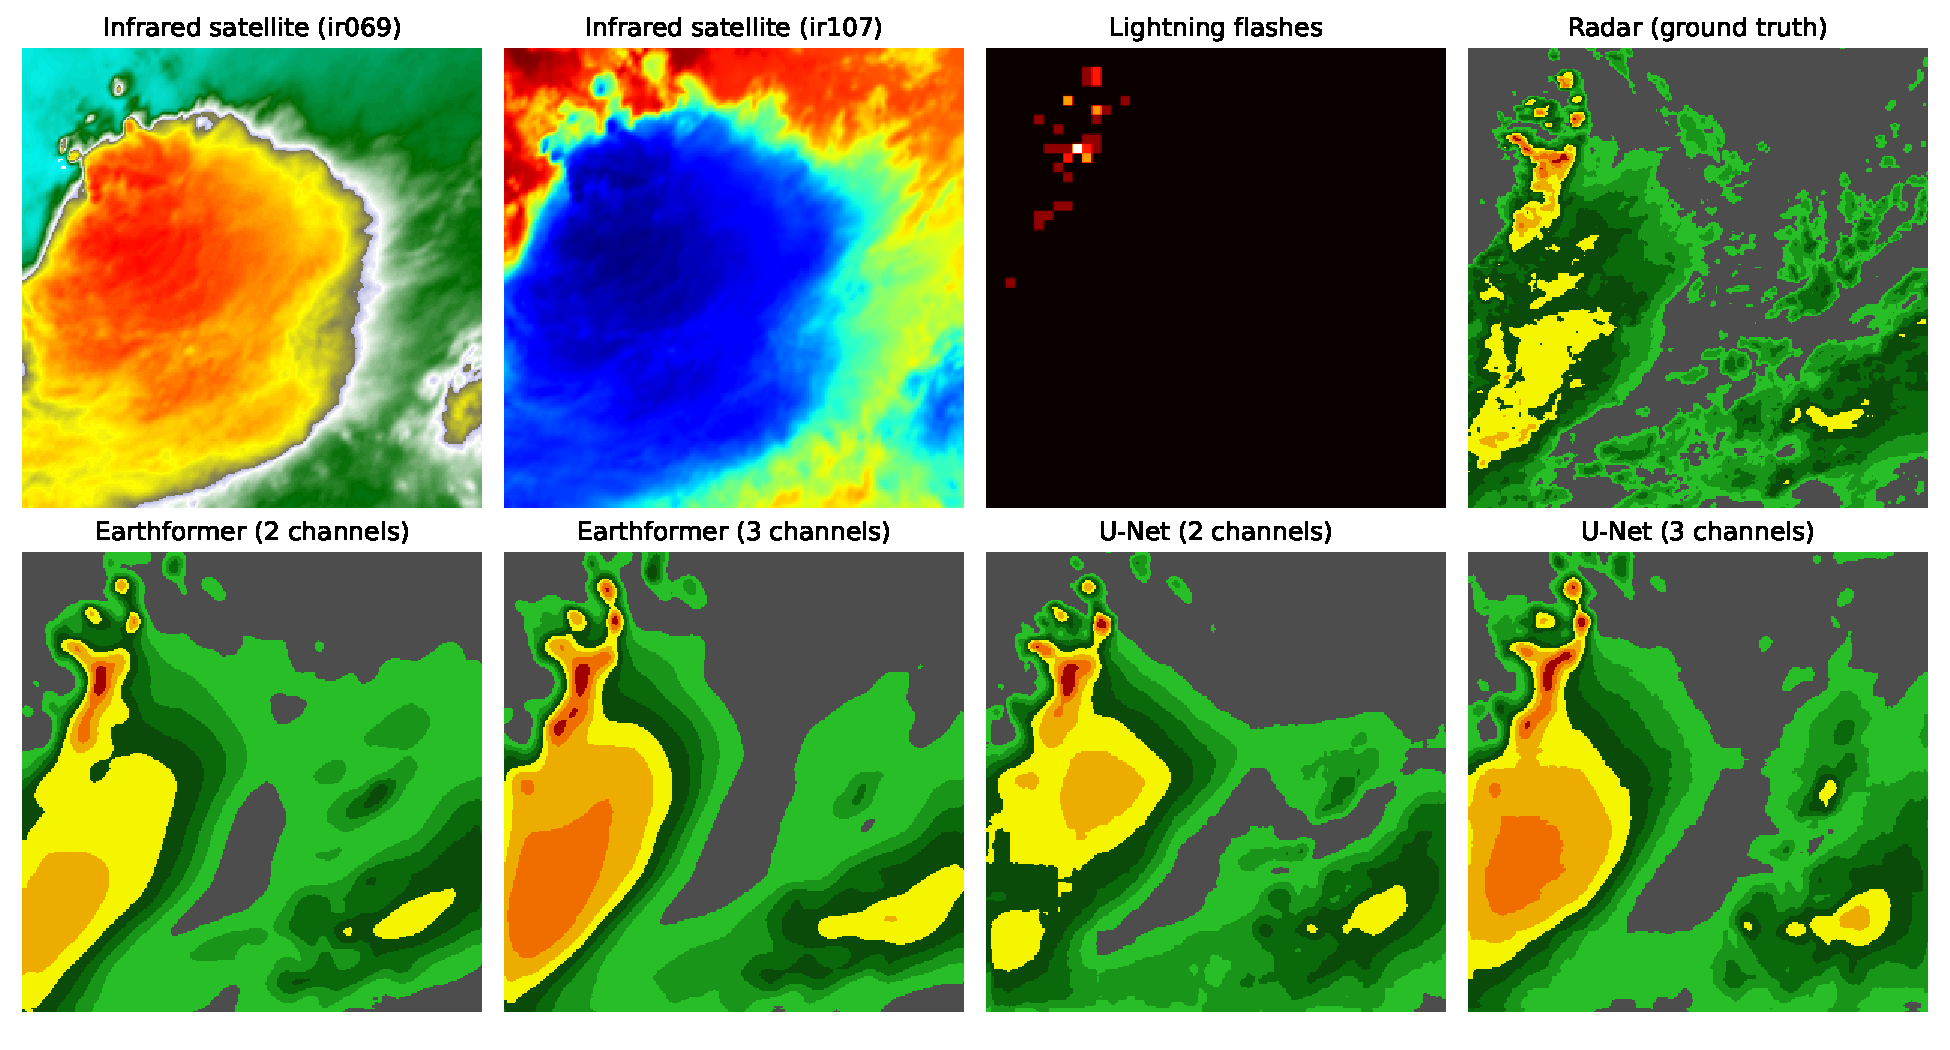
\includegraphics[width=\linewidth]{img/examples.pdf}
  \caption{Example visualizations of the input and target channels (top row) and the predicted radar outputs (bottom row).}
  \label{fig:predictions}
\end{figure*}


%%%%%%%%%%%%%%%%%%%%%%%%%%%%%%%%%%%%%%%%%%%%%%%%%%%%%%%%%%%%%%%%%%%%%%%%%%%%%%%%
\section{Conclusion and discussion}
In this work, we utilized the Earthformer model for predicting synthetic radar images from satellite images using the SEVIR dataset. The Earthformer was able to successfully extract rainfall data from the satellite inputs with comparable performance to a U-Net model. When trained with MSE loss, the Earthformer achieved the lowest MAE, while the U-Net had the best MSE and CSI. For training with MAE, the U-Net outperformed Earthformer in all three metrics. We also showed that incorporating lightning flashes into the input data improves the predictions both quantitatively and visually, helping the models predict high-intensity precipitation.

Both our models showcased potential for further use in other meteorological tasks. By adjusting our models to allow for sequence prediction, they could be used for precipitation nowcasting in parts of the world without ground radars.

While we showed the capabilities of the Earthformer for sat2rad translation, our work comes with many limitations. Most significantly, the hyperparameter search was very limited and a more thorough exploration could have yielded better results. Further research could also focus on adjusting the training procedure and loss engineering.

%%%%%%%%%%%%%%%%%%%%%%%%%%%%%%%%%%%%%%%%%%%%%%%%%%%%%%%%%%%%%%%%%%%%%%%%%%%%%%%%
\printbibliography

\end{document}
